\chapter{Future Work}

With this work we barely scratched the surface of what can be done with CCH in neo4j. 
There are a lot of special topics one could dive deeper to improve CCH for neo4j.

\section{Contraction Algorithms}

As the contraction algorithm \ref{alg:contraction} we use definitely has its limitation as we have seen in the experiment section \ref{sec:contraction_limits}, it is worth digging
deeper there. One very promising method determine the vertex by recursively look for minimum balanced separators until they tend to get big and then continue with our algorithm.
Another question we haven't even touched is, what if we add vertices and arcs. How can we deal with such updates in the input graph which are not unusual for databases.

\section{The Test Dataset}

Changing the test domain can be interesting, too. Most papers like \cite[CCH]{CCH}, and \cite[CH]{Geisberger_2012} and many more focus on road networks. This definitely made sense for this
paper to also check if we come to similar results. However, one could also try grids as \cite[Storandt]{storandt2013contraction} or looking for other real world domains that can be modeled such that shortest path queries are of major interest.

\section{Perfect Customization and Transition to CH}

\begin{wrapfigure}{r}{0.5\textwidth}
    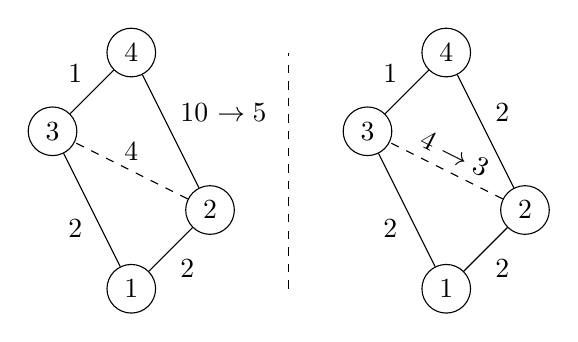
\begin{tikzpicture}[node distance={15mm}, main/.style = {draw, circle}]

    \node[main] (x3) at (0, 2) {$3$};
    \node[main] (x4) at (1, 3) {$4$};
    \node[main] (x2) at (2, 1) {$2$};
    \node[main] (x1) at (1, 0) {$1$};
    
    \draw (x1) -- node[below right] {$2$}(x2);
    \draw (x1) -- node[below left] {$2$} (x3);
    \draw (x2) -- node[above right] {\sout{$10$} $\rightarrow 5$} (x4);
    \draw (x3) -- node[above left] {$1$} (x4);
    \draw[dashed] (x2) -- node[above] {$4$} (x3);

    \draw[dashed]  (3,0) -- (3,3);

    \node[main] (x31) at (4, 2) {$3$};
    \node[main] (x41) at (5, 3) {$4$};
    \node[main] (x21) at (6, 1) {$2$};
    \node[main] (x11) at (5, 0) {$1$};
    
    \draw (x11) -- node[below right] {$2$}(x21);
    \draw (x11) -- node[below left] {$2$} (x31);
    \draw (x21) -- node[above right] {$2$} (x41);
    \draw (x31) -- node[above left] {$1$} (x41);
    \draw[dashed] (x21) -- node[above, sloped] {\sout{$4$} $\rightarrow 3$}  (x31);

    
\end{tikzpicture}
    
\end{wrapfigure}

We didn't implement the perfect customization, nor the transition from CCH to CH. A CH index is usually faster at query time as the amount of arcs is less. Therefore it can be useful to have 
a CCH and always calculate a CH from it after each update. In that scenario it is also useful to measure how long such a transition takes.

\section{Using relational Databases}

Furthermore it is questionable if graph databases like neo4J solve any problem. Due to \cite[The Case Against Specialized Graph Analytics Engines]{fan2015case} there is no significant difference in processing a graph in a graph database compared to a relational 
database. Therefore it would be interesting to see, how an implementation of dijkstra and (C)CH perform in SQL, written for relational databases. 